% Template for PLoS
% Version 3.5 March 2018
%
% % % % % % % % % % % % % % % % % % % % % %
%
% -- IMPORTANT NOTE
%
% This template contains comments intended 
% to minimize problems and delays during our production 
% process. Please follow the template instructions
% whenever possible.
%
% % % % % % % % % % % % % % % % % % % % % % % 
%
% Once your paper is accepted for publication, 
% PLEASE REMOVE ALL TRACKED CHANGES in this file 
% and leave only the final text of your manuscript. 
% PLOS recommends the use of latexdiff to track changes during review, as this will help to maintain a clean tex file.
% Visit https://www.ctan.org/pkg/latexdiff?lang=en for info or contact us at latex@plos.org.
%
%
% There are no restrictions on package use within the LaTeX files except that 
% no packages listed in the template may be deleted.
%
% Please do not include colors or graphics in the text.
%
% The manuscript LaTeX source should be contained within a single file (do not use \input, \externaldocument, or similar commands).
%
% % % % % % % % % % % % % % % % % % % % % % %
%
% -- FIGURES AND TABLES
%
% Please include tables/figure captions directly after the paragraph where they are first cited in the text.
%
% DO NOT INCLUDE GRAPHICS IN YOUR MANUSCRIPT
% - Figures should be uploaded separately from your manuscript file. 
% - Figures generated using LaTeX should be extracted and removed from the PDF before submission. 
% - Figures containing multiple panels/subfigures must be combined into one image file before submission.
% For figure citations, please use "Fig" instead of "Figure".
% See http://journals.plos.org/plosone/s/figures for PLOS figure guidelines.
%
% Tables should be cell-based and may not contain:
% - spacing/line breaks within cells to alter layout or alignment
% - do not nest tabular environments (no tabular environments within tabular environments)
% - no graphics or colored text (cell background color/shading OK)
% See http://journals.plos.org/plosone/s/tables for table guidelines.
%
% For tables that exceed the width of the text column, use the adjustwidth environment as illustrated in the example table in text below.
%
% % % % % % % % % % % % % % % % % % % % % % % %
%
% -- EQUATIONS, MATH SYMBOLS, SUBSCRIPTS, AND SUPERSCRIPTS
%
% IMPORTANT
% Below are a few tips to help format your equations and other special characters according to our specifications. For more tips to help reduce the possibility of formatting errors during conversion, please see our LaTeX guidelines at http://journals.plos.org/plosone/s/latex
%
% For inline equations, please be sure to include all portions of an equation in the math environment.  For example, x$^2$ is incorrect; this should be formatted as $x^2$ (or $\mathrm{x}^2$ if the romanized font is desired).
%
% Do not include text that is not math in the math environment. For example, CO2 should be written as CO\textsubscript{2} instead of CO$_2$.
%
% Please add line breaks to long display equations when possible in order to fit size of the column. 
%
% For inline equations, please do not include punctuation (commas, etc) within the math environment unless this is part of the equation.
%
% When adding superscript or subscripts outside of brackets/braces, please group using {}.  For example, change "[U(D,E,\gamma)]^2" to "{[U(D,E,\gamma)]}^2". 
%
% Do not use \cal for caligraphic font.  Instead, use \mathcal{}
%
% % % % % % % % % % % % % % % % % % % % % % % % 
%
% Please contact latex@plos.org with any questions.
%
% % % % % % % % % % % % % % % % % % % % % % % %

\documentclass[10pt,letterpaper]{article}
\usepackage[top=0.85in,left=2.75in,footskip=0.75in]{geometry}

% amsmath and amssymb packages, useful for mathematical formulas and symbols
\usepackage{amsmath,amssymb}

% Use adjustwidth environment to exceed column width (see example table in text)
\usepackage{changepage}

% Use Unicode characters when possible
\usepackage[utf8x]{inputenc}

% textcomp package and marvosym package for additional characters
\usepackage{textcomp,marvosym}

% cite package, to clean up citations in the main text. Do not remove.
\usepackage{cite}

% Use nameref to cite supporting information files (see Supporting Information section for more info)
\usepackage{nameref,hyperref}

% line numbers
\usepackage[right]{lineno}

% ligatures disabled
\usepackage{microtype}
\DisableLigatures[f]{encoding = *, family = * }

% color can be used to apply background shading to table cells only
\usepackage[table]{xcolor}

% array package and thick rules for tables
\usepackage{array}

% create "+" rule type for thick vertical lines
\newcolumntype{+}{!{\vrule width 2pt}}

% create \thickcline for thick horizontal lines of variable length
\newlength\savedwidth
\newcommand\thickcline[1]{%
  \noalign{\global\savedwidth\arrayrulewidth\global\arrayrulewidth 2pt}%
  \cline{#1}%
  \noalign{\vskip\arrayrulewidth}%
  \noalign{\global\arrayrulewidth\savedwidth}%
}

% \thickhline command for thick horizontal lines that span the table
\newcommand\thickhline{\noalign{\global\savedwidth\arrayrulewidth\global\arrayrulewidth 2pt}%
\hline
\noalign{\global\arrayrulewidth\savedwidth}}



%%  Packages added by Colin
% Symbols
\usepackage{amsmath,amssymb,url,bm}
% Formatting
\usepackage{multicol, csquotes, scrextend, color}   %, titlesec
%% Tables, Figures
\usepackage{longtable, booktabs, pdflscape, placeins}

% Images
\usepackage{graphicx, float, caption, subcaption}

% package added by Oster for editing
\usepackage{color} 
\newcommand{\red}[1]{{\color{red}{#1}}}





% Remove comment for double spacing
%\usepackage{setspace} 
%\doublespacing

% Text layout
\raggedright
\setlength{\parindent}{0.5cm}
\textwidth 5.25in 
\textheight 8.75in

% Bold the 'Figure #' in the caption and separate it from the title/caption with a period
% Captions will be left justified
\usepackage[aboveskip=1pt,labelfont=bf,labelsep=period,justification=raggedright,singlelinecheck=off]{caption}
\renewcommand{\figurename}{Fig}

% Use the PLoS provided BiBTeX style
% Colin commented this out - added where bibliography is inserted
% \bibliographystyle{plos2015}

% Remove brackets from numbering in List of References
\makeatletter
\renewcommand{\@biblabel}[1]{\quad#1.}
\makeatother

% Header and Footer with logo
\usepackage{lastpage,fancyhdr,graphicx}
\usepackage{epstopdf}
%\pagestyle{myheadings}
\pagestyle{fancy}
\fancyhf{}
%\setlength{\headheight}{27.023pt}
%\lhead{\includegraphics[width=2.0in]{PLOS-submission.eps}}
\rfoot{\thepage/\pageref{LastPage}}
\renewcommand{\headrulewidth}{0pt}
\renewcommand{\footrule}{\hrule height 2pt \vspace{2mm}}
\fancyheadoffset[L]{2.25in}
\fancyfootoffset[L]{2.25in}
\lfoot{\today}

%% Include all macros below

\newcommand{\lorem}{{\bf LOREM}}
\newcommand{\ipsum}{{\bf IPSUM}}

%% END MACROS SECTION


\begin{document}
\vspace*{0.2in}

% Title must be 250 characters or less.
\begin{flushleft}
{\Large
\textbf\newline{Prediction of homelessness risk based on utility payment history} % Please use "sentence case" for title and headings (capitalize only the first word in a title (or heading), the first word in a subtitle (or subheading), and any proper nouns).
}
\newline
% Insert author names, affiliations and corresponding author email (do not include titles, positions, or degrees).
\\
Colin D.\ Middleton\textsuperscript{1},
Andrew M.\ Oster\textsuperscript{1*} \\
\bigskip
\textbf{1} Department of Mathematics, Eastern Washington University, Cheney, WA, USA
\\

\bigskip


% Current address notes
%\textcurrency Current Address: Dept/Program/Center, Institution Name, City, State, Country % change symbol to "\textcurrency a" if more than one current address note
% \textcurrency b Insert second current address 
% \textcurrency c Insert third current address

% Deceased author note
%\dag Deceased

% Group/Consortium Author Note
%\textpilcrow Membership list can be found in the Acknowledgments section.

% Use the asterisk to denote corresponding authorship and provide email address in note below.
*aoster@ewu.edu

\end{flushleft}
% Please keep the abstract below 300 words
\section*{Abstract}
In order to reduce homeless numbers in Spokane County, the City of Spokane, Avista Utilities, Urbanova, Eastern Washington University and Washington State University formed a consortium, the Spokane Predictive Analytics Group, to collect data to develop new predictive tools to identify those at risk of homelessness.  In this work, we present results from de-identified 


Both the City of Spokane and Avista Utilities provided de-identified data 


% Please keep the Author Summary between 150 and 200 words
% Use first person. PLOS ONE authors please skip this step. 
% Author Summary not valid for PLOS ONE submissions.   
%\section*{Author summary}

%%   \linenumbers    -- use 

% Use "Eq" instead of "Equation" for equation citations.


\section*{Introduction}
\subsection*{Problem}
In order to reduce homeless numbers in Spokane County, the City of Spokane, Avista Utilities, Urbanova, Eastern Washington University an Washington State University formed a consortium, the Spokane Predictive Analytics Group, to determine if utility customer billing data is useful for predicting homelessness and to develop new predictive tools to identify those at risk of homelessness.  Both the City of Spokane and Avista Utilities provided de-identified data.

% Definition of Homelessness
The Department of Housing and Urban Development has categories of homelessness and define their \textit{``Category 1: Literally Homeless"} to be
\begin{displayquote}[~\cite{hud_hmls_def}]
1) Individual or family who lacks a fixed, regular, and adequate nighttime residence, meaning: \\
(i) Has a primary nighttime residence that is a public or private place not meant for human habitation; \\
(ii) Is living in a publicly or privately operated shelter designated to provide temporary living arrangements (including congregate shelters, transitional housing, and hotels and motels paid for by charitable organizations or by federal, state and local government programs); or \\
(iii) Is exiting an institution where (s)he has resided for 90 days or less and who resided in an emergency shelter or place not meant for human habitation immediately before entering that institution
\end{displayquote}

The agencies that collected the data utilized in this work used HUD's \textit{``Category 1: Literally Homeless"} definition of homeless, and in this work we adopt that definition.

\subsubsection*{The Current State of Homelessness}
Homelessness in the United States persists despite the efforts of \red{PROGRAMS} and \red{MONEY, MONEY spent each year} on assistance programs.  From 2005 until 2020, impressively there has been a decrease of 42\% in homelessness in the USA according to the Department of Housing and Urban Development (HUD).  Regretfully, HUD still reported over 442,000 people experiencing homelessness in 2020 through their Point in Time Count program ~\cite{PITcount}.   \red{ Is there data that shows a rise in homelessness?  Or a recent rise in light of the pandemic???}

In this work, we consider homelessness in Spokane County, Washington, USA.  Spokane County has seen  homelessness levels decrease by 32\% from 2005 to 2020 with 1,244 people recorded as experiencing homelessness in 2020 ~\cite{PITcount}. These numbers include individuals sheltered in emergency shelters, sheltered in transitional housing, and unsheltered ~\cite{PITcount}, however \red{some fear PIT counts far underestimate homeless numbers*****}.  

%  Washington State has seen a decrease in homelessness of 28\% from 2005 to 2020, but according to HUD still retains over 17,000 people experiencing homelessness.

\begin{figure}[H]
    \begin{minipage}{0.5\textwidth}
        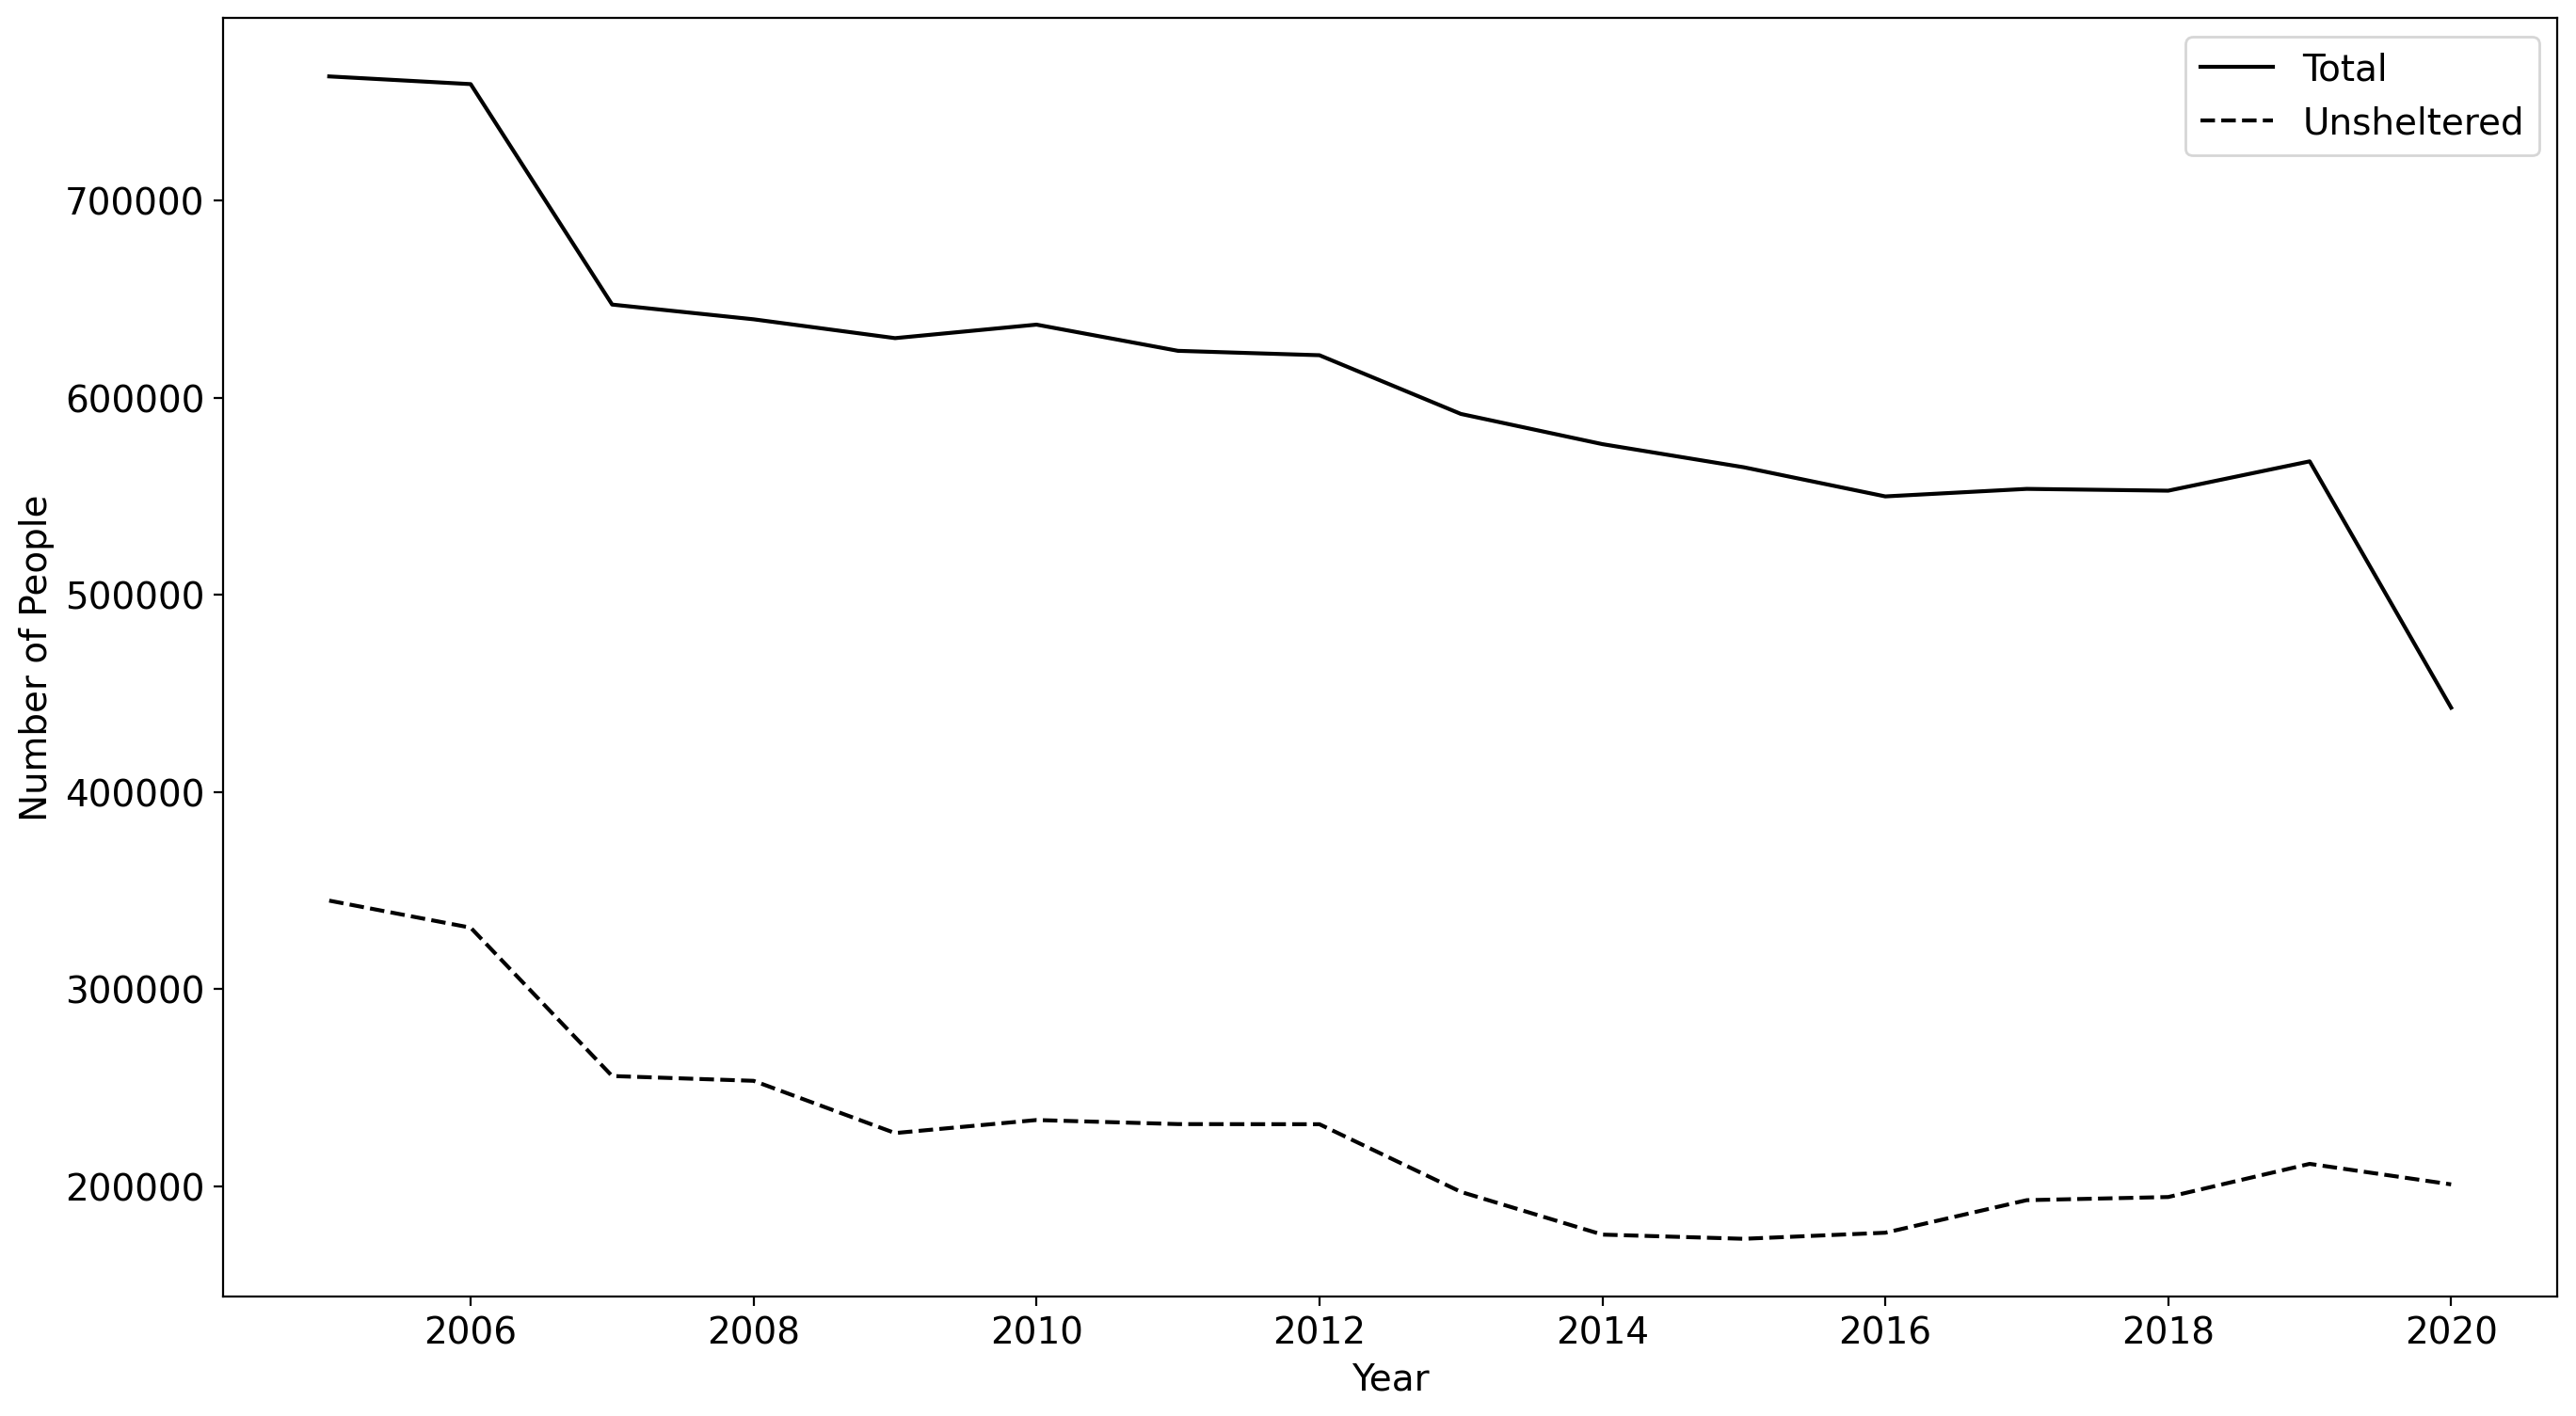
\includegraphics[width=\textwidth]{../img/homelessness_usa.png} 
    \end{minipage}
    \begin{minipage}{0.5\textwidth}
        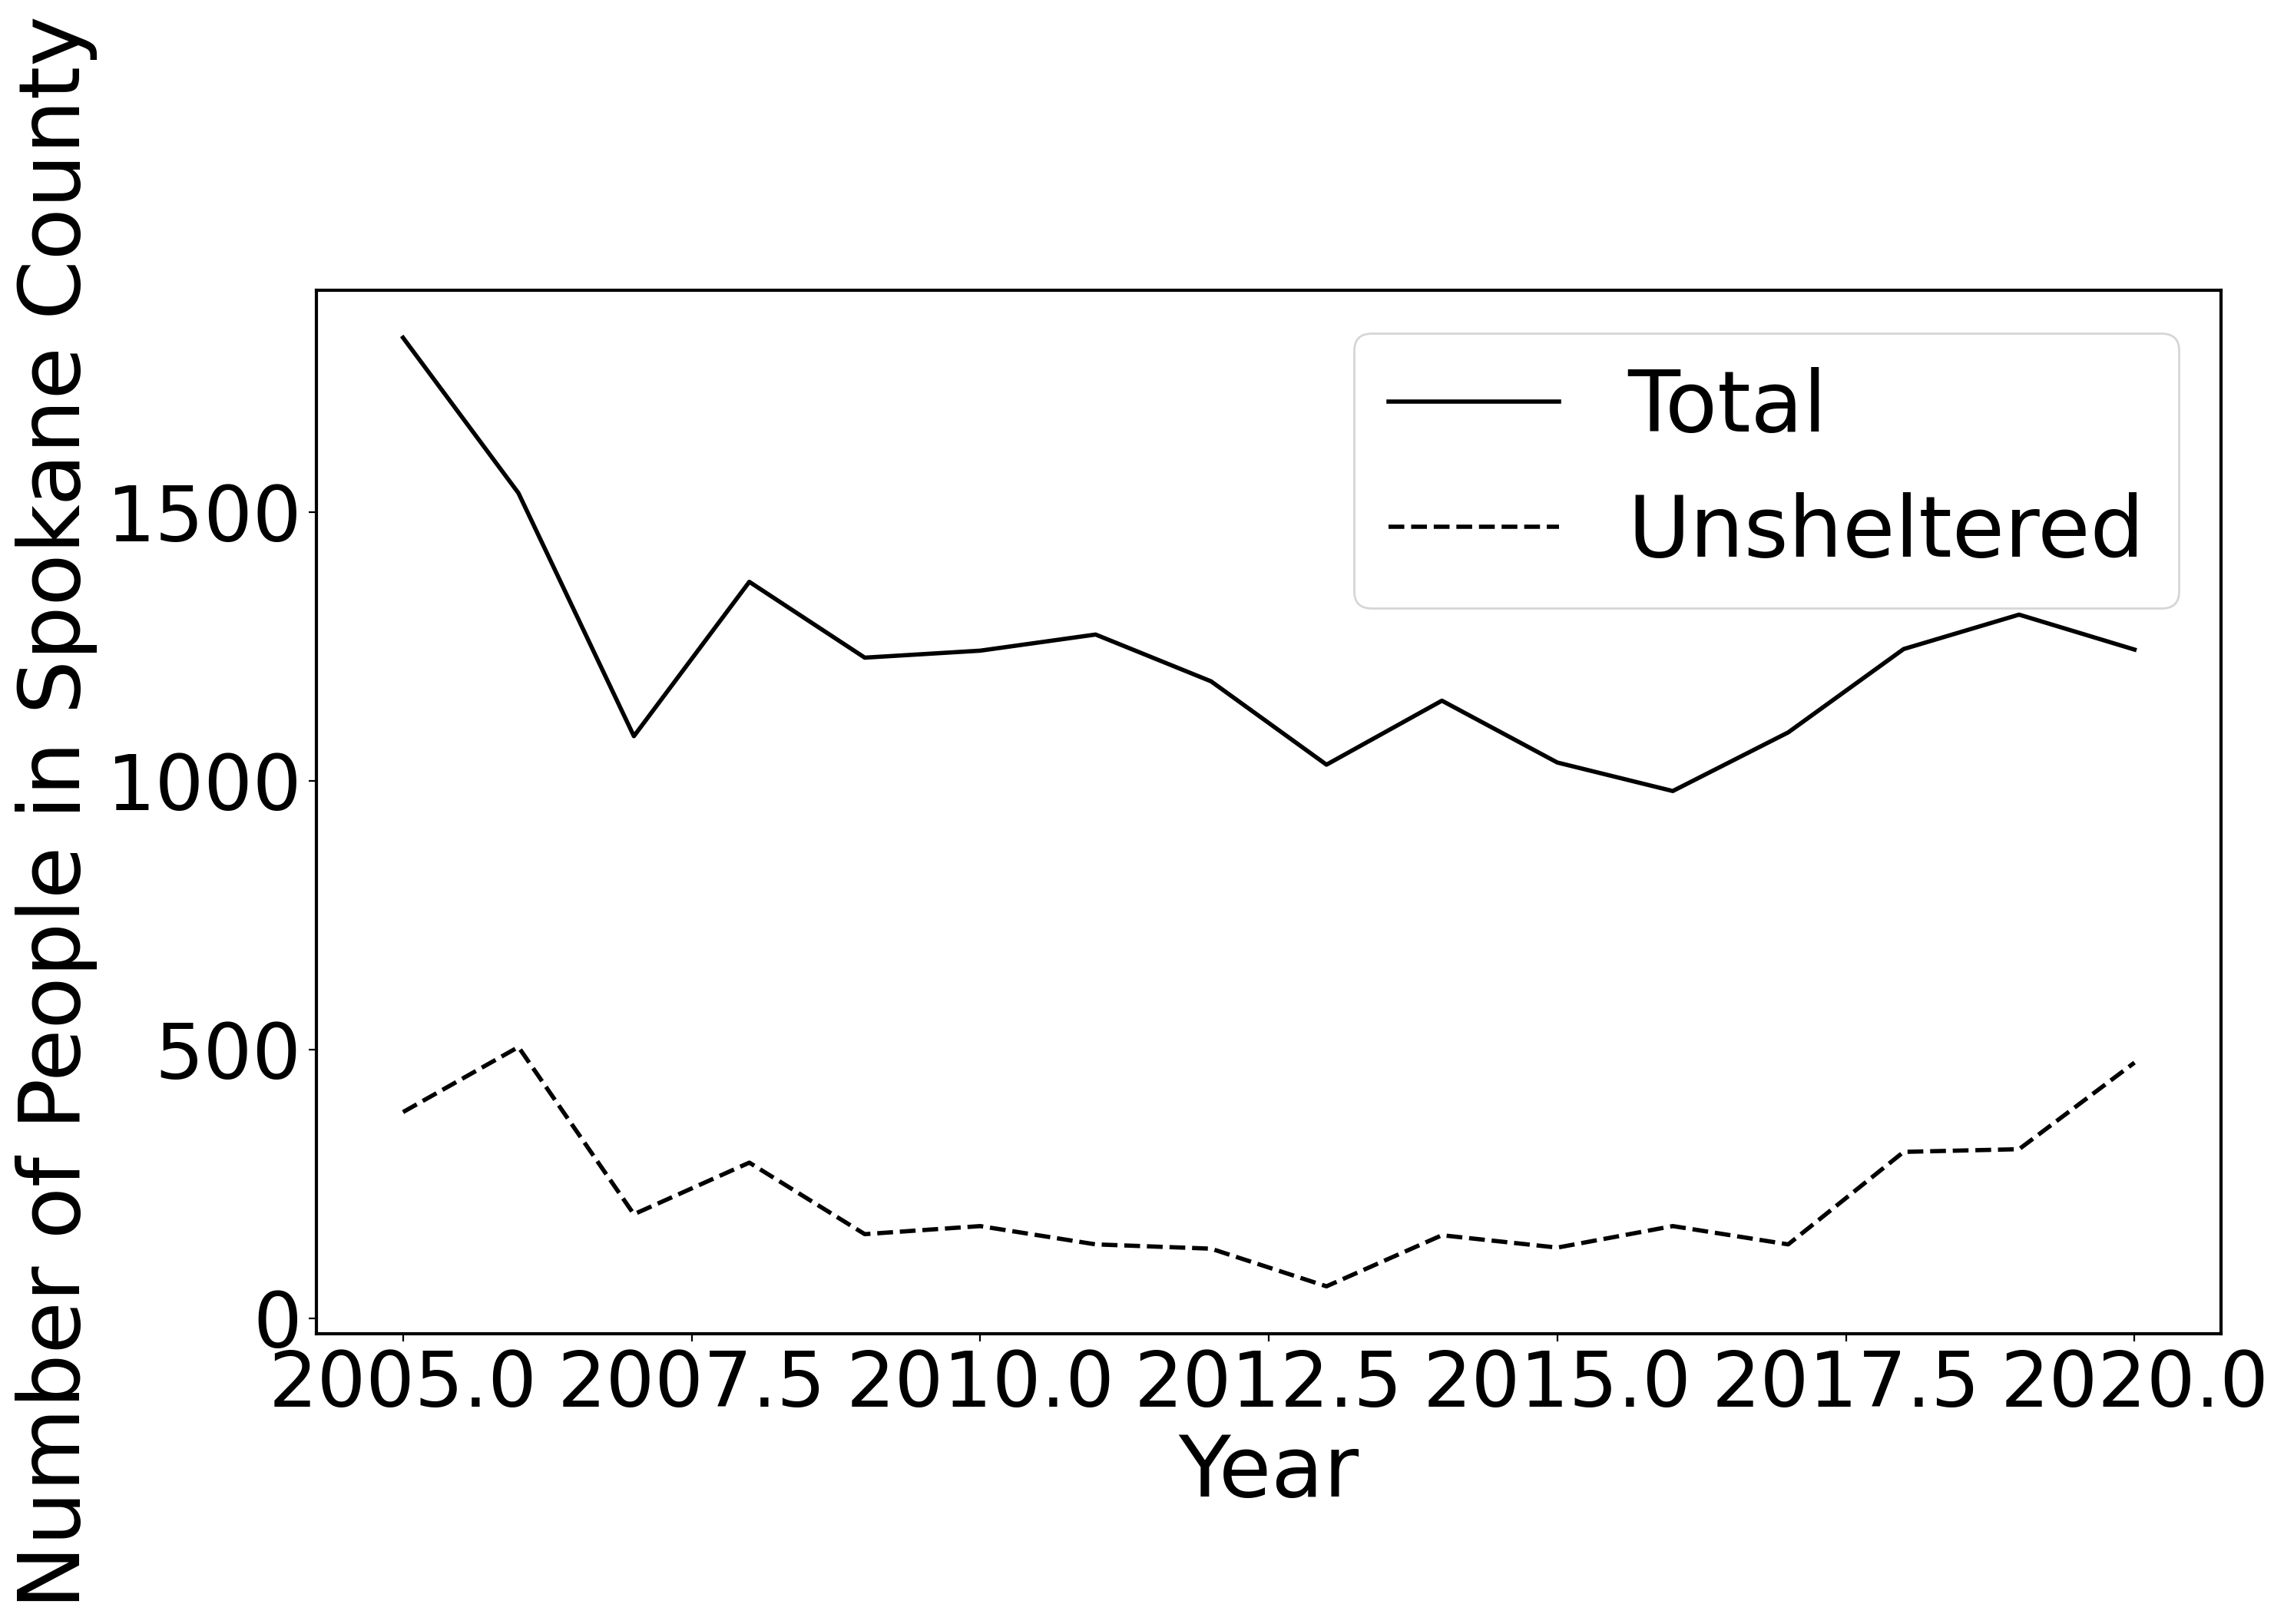
\includegraphics[width=\textwidth]{../img/homelessness_spokane.png}
    \end{minipage}
    \caption[Annual Homelessness Counts in the USA and Spokane County]{Annual Homelessness Counts in the USA and Spokane County
    ~\cite{PITcount}   \\ \red{font size need to be far larger on axes, perhaps thicker lines in plots}    }
    \label{fig:Homeless_US_Spokane}
\end{figure}

% Efforts to combat homelessness
Programs focused on providing assistance to people experiencing homelessness are having an impact. HUD's January 2019 survey found that ``there were 144,000 more permanent supportive housing (PSH) beds dedicated to people with chronic patterns of homelessness than there were in 2007 (a 380\% increase)'' ~\cite{2019AHAR}. Likely because of this increase in resources the rate of chronic homelessness (people who have experienced homelessness for at least 12 months in the last three years) has declined by 20\% from 2007 to 2019 in the US~\cite{2019AHAR}. Current assistance programs and the positive impacts they have on people in need represent a significant accomplishment, but these programs largely focus on providing support to people already experiencing homelessness. This type of assistance program can only help so much. In order to substantially reduce and eventually end homelessness altogether, homelessness prevention programs must be utilized. 

We will refer to programs as homelessness prevention programs (HPPs) if they focus on preventing people from experiencing homelessness. These programs include permanent deep rental housing subsidies, eviction prevention programs, community based services such as short term financial assistance, education, and job placement. Homeless assistance programs (HAPs), we shall say are those that are specifically aimed at assisting people who are currently experiencing an episode of homelessness and include shelters and other emergency services. There are two aspects of HPPs that make them more attractive than HAPs. The first is cost. The services that HPPs typically offer are less expensive for taxpayers than those provided by HAPs ~\cite{shinn2019homelessness}. The second reason is that if the HPP is successful it will spare people the trauma typical of experiencing homelessness.

\subsubsection*{Cost Effectiveness of Homeless Prevention Programs}
Research has shown that many types of HPPs are cost effective in practice, meaning that treating the social issue of homelessness with HPPs instead of HAPs in the same area is at least as effective at keeping people off the streets and costs less money. This is due to the high cost of HAPs - once someone experiences an episode of homelessness, they often use high-cost services such as shelters and emergency health services \red{add source}.

A study on permanent deep rental housing subsidies, one of the most promising types of HPP, found that ``among the 67 percent of families who successfully used their [rent subsidy] voucher to lease housing, homelessness was prevented entirely'' ~\cite{shinn2019homelessness} (Page 5). Another study analyzed an eviction prevention program from 2010 to 2012 in Chicago that distributed rent assistance based on at-risk individuals calling a Homelessness Prevention Call Center. Researchers found that six months after a person had called in, only 0.5\% of those who received financial aid experienced homelessness, while 2.1\% of those who did not receive aid experienced homelessness. The program was especially helpful for the lowest income callers and the authors claim could have been more efficient with better targeting ~\cite{evans2016impact}. In New York City a program called HomeBase provides community based services to at-risk individuals. Two papers have concluded that this program is cost effective at preventing homelessness ~\cite{rolston2013evaluation} ~\cite{goodman2016homelessness}. 

Homeless prevention is effective on a large scale as well. In 2009 the United States government distributed \$1.5 billion through the Homeless Prevention and Rapid Rehousing Program which promoted HPPs. According to the National Alliance to End Homelessness this spending and promotion of HPPs largely caused the 1\% decline in homelessness between 2009 and 2011, which is notable considering the economic recession during that time ~\cite{shinn2013efficient}.

% The pathology of homelessness
There is one important aspect of the pathology of homelessnes that is likely the cause of HPPs' effectiveness - a gradual divergence from financial stability. We hypothesise that individuals that eventually experience homelessness begin thier journey as indistinguishable from the healthy population. As time moves forward, these individuals begin to shows signs of financial distress and become more and more separate from the healthy population (and more identifiable as at-risk) as they progress towards experiencing homelessnes. As this progression occurs, and especially once an individual experiences an episode of homelessness, it becomes more difficult to change their financial trajectory and help them reestablish their independence. This hypothesis is supported by Shinn's ``Efficient Targeting of Homelessness Prevention Services for Families,'' which found that ``[t]he single best predictor of eventual homelessness is having previously been in a shelter'' ~\cite{shinn2019homelessness} (Page 3). The point of HPPs is to change the trajectories of at-risk individuals early in this process. If an intervention is performed early in the process, only a minor course correction is necessary. 

% No one is too high-risk to assist
There does not appear to be any significant portion of the population that is too high-risk for HPPs to assist. In a study on New York's HomeBase program in 2013 it was found that ``No level of risk was too high for families to benefit from services and, indeed, even in the highest decile of measured risk, a majority of families avoided shelter'' ~\cite{shinn2013efficient} (Page 3). This finding is important because it provides statistical backing to the notion that no one is beyond help. It also informs which part of the population HPPs should focus on - people who are predicted to have the highest risk of experiencing homelessness.

According to a 2019 study by the California Policy Lab, HPPs should be both effective and efficient. An \textit{effective} program prevents people from experiencing homelessness that would have if they had not been provided assistance. An \textit{efficient} program only provides assistance to those who actually need it ~\cite{PredictPreventHmlsnsLA}. A good analogy here is that HPPs striving to provide assistance to a certain type of person, those who will experience homelessness, is like casting a net to catch a certain type of fish. Programs that ``cast a large net'' by assisting many people can easily be effective because they are likely to prevent a large number of people from experiencing homelessness. However, it is difficult for such a program to be efficient because it will inevitably provide assistance to many people who would not experience homelessness even if they did not receive assistance. In a similar way a program that ``casts a small net,'' targeting the people identified as most at-risk of experiencing homelessness, can be highly efficient by only providing assistance to people who would have experienced homelessness, but is likely less effective because some people who do not receive assistance will still experience homelessness simply because they were not identified as the most at-risk. The ideal situation is a program that assists all the people who would experience homelessness and none who would not. This ideal is almost certainly unattainable in practice due to the difficulty of identifying who will experience homelessness. The key to providing this targeted assistance is correctly identifying the most at-risk individuals and doing so as early as possible in order to give them the best chance at correcting their trajectory.

\subsubsection*{Predicting Homelessness}
Identifying individuals to enroll in HPPs is a difficult task because everyone is a candidate; anyone might experience homelessness at some point in the future. The path to homelessness may be different for different individuals and people may persist in a high-risk-of-homelessness state without ever experiencing an episode of homelessness. Only when a tipping point is reached - one too many bills are due close together, a parking ticket, a medical expense, etc. - does someone lose their housing and experience an episode of homelessness ~\cite{o2004wrong}. Because of this ability for some individuals to maintain a state of financial distress but never experience homelessness, even the best prediction models will likely produce false positives, that is, predict some people as having a high risk of experiencing homelessness when they never actually do.

Currently, screening for HPPs is almost entirely performed by healthcare workers. Using surveys, their experience, and their intuition they evaluate each individual and determine who gets which aid and how much. There are at times high volumes of individuals seeking assistance, especially in large cities, which slows down this system. Another issue is that the evaluators have biases which may affect their decisions about who gets aid and who does not ~\cite{shinn2019homelessness}.

The use of statistical models as a screening method shows promise in this area. Statistical models add more objectivity to the screening process; any bias they contain can be measured and corrected. One study found that the use of a screening model reduced the number of applicants to HPPs who were turned down and then eventually entered a shelter from 28.4\% to 8.1\% ~\cite{shinn2019homelessness}. Screening systems using statistical models are also fast and easily automated which reduces the burden on healthcare workers, are less expensive to operate, and can help speed up the overall process of providing assistance to those in need.

\subsection*{Goals}
The main goal of this study is to determine if ubiquitous information contained in utility customer billing data is useful in predicting first time homelessness. We accomplish this analysis by using some of this data that is locally available, but could be found anywhere across the US, to train a statistical model and predict first time homelessness, then evaluate the model's effectiveness.

% Determine usefulness of utility customer billing data for predicting homelessness
Our project uses utility customer payment data to predict risk of experiencing homelessness. This data source is attractive for two key reasons. First, it contains information related to individuals' financial health such as utility bill amounts, amount owed to the utility company, and number of times a bill payment was missed. Risk of homelessness is closely linked with an individual's financial health.

The second reason why utility data is attractive is its ubiquity. Almost all households pay some form of utility bill, so this data is available for nearly everyone across the U.S. It may exist in different forms and in different agencies, but similar information on amounts owed and payment default likely exists in all utility-customer situations. If it were a source of useful information in predicting homelessness, any derived models could be used anywhere in the U.S. using similar data sources. 

% Create model that produces few false-negatives
The intention is to combine the utility data, if useful, with other known sources of useful information in predicting homelessness to create the most effective prediction model possible. However, our model could be used to predict homelessness with only the utility data. A convenient model output format, and the one chosen for this project, is a ranked list of individuals and their associated risks of experiencing homelessness. With this information, the HPP using the model can assist at-risk individuals in two convenient ways: \red{remove this?}

\begin{itemize}
    \item Option 1
    \begin{enumerate}
        \item Assess the pool of resources available to assist at-risk individuals,
        \item determine the number of people that can receive aid based on this pool, say $n$,
        \item and simply choose the $n$ individuals with highest predicted risk.
    \end{enumerate}
    \item Option 2
    \begin{enumerate}
        \item Analyze the list of individuals and their risks of experiencing homelessness,
        \item choose a threshold risk value,
        \item then assist all individuals above that threshold. This method may be appropriate if there is a large gap in predicted risks.
    \end{enumerate}
\end{itemize}


\subsection*{Precedent Research}
\subsubsection*{Data Sources}
Most other studies do not predict homelessness on the entire population but instead focus on more at-risk subpopulations. 

Used other data sources: health, DOJ, other assistance services

\subsubsection*{Models}
logistic regression, cox regression, atrificial neural network, points-based questionaire

\subsubsection*{Performance Evaluation}
Reporting on model performance varies significantly from study to study.

\subsection*{Our Contribution}
Call for standardized model performance reporting. 

Determine usefulness of ubiquitous utility customer billing data.

Present a model that performs well compared to current research that relies only on ubiquitous utility billing data.


%------------------- Materials and Methods ---------------------------------
\section*{Materials and Methods}
\subsection*{The Data}
% Sources
The data used for this project was obtained from Avista Utilities and the City of Spokane. Avista Utilities provided monthly residential customer billing information for electricity and natural gas utilities. The City of Spokanen provided monthly combined water, sewer, and garbage billing information as well as outcome data on who has been recorded as experiencing homelessness and at what times.

\subsubsection*{Data Preperation}
% Data Imbalance
The high degree of imbalance in the dataset, that is, the large number of negative cases, people who were never recorded as experiencing homelessness within the dataset, compared to the small number of positive cases, people who were recorded as experiencing homelessness, was a major challenge to model fitting. Specifically, there were 302 positive cases and 84,066 negative cases. This imbalance adds difficulty to the model's task of distinguishing between positive and negative cases because it is difficult to identify the few positive cases among the many negative cases, especially if there are many negative cases that are similar to the positive cases. In this study identifying the positive cases in the dataset is much more important than the negative cases.

% Matching + De-Identifying
Initial data matching and de-identifying was performed by the data team at Avista Utilities. This process involved gathering the data from its sources and matching on name, address, and month. After matching, the data was de-identified by replacing any identifiable characteristics of the data such as name and address with internally generated identification numbers. Additional matching was performed by the authors. After this process, the data contained information on 85,345 people who have been listed as the main account holder on a utility billing account in Spokane County from December, 2015 to December, 2020. For each person there are monthly entries with information about thier utility billing activities. 

% Association Metrics
To measure relationships between variables in the data, different association metrics were used depending on the variable types. The following is a list of variable pairing types and the metric used to measure strength of association between the variables: absolute value of Spearman Correlation for continuous-continuous, Point-Biserial Correlation for binary-continuous, Theil Uncertainty Coefficient for categorical-categorical, and Correlation Ratio for continuous-categorical(with more than two levels). \red{REMOVE PREVIOUS PAGARAPH?}

% Data Homogeneity
\red{MOVE BELOW PART TO DISCUSSION?}
When attempting to learn patterns and relationships from data, it is important to understand if certain parts of the data are different from other parts. For this project we are distinguishing between positive (someone who has experienced homelessness) and negative (someone who has not experienced homelessness) cases, but the relationships between the predictor variables and the outcome may change over time. Perhaps there were different relationships between the predictor variables and homelessness during different years. 

The year 2020 was expected to contain different relationships than the previous years because the COVID-19 pandemic caused people and the utility agencies to behave differently than they had in previous years. For example, for the greater part of 2020, the utility agencies tracked in our dataset did not perform service shut-offs as they had in previous years \cite{white2020utilities}. 

To investigate if there was a difference in the associations between the variables and the outcome in different years, the data was split by year, the strength of association of each variable with the outcome (CMIS\_MATCH) was measured, these strengths were then ranked, and the rankings were compared from year to year. Table~\ref{tbl:corr_years} displays these rankings. Surprisingly, they appear to be very similar from year to year. This means that the important relationships within the data are similar from year to year, so all available years, 2015 to 2020, were included in further analysis and modeling.

\begin{table}[!h]
    \centering
    \begin{tabular}{lcccccc}
        \toprule
                 Variable &  2015 &  2016 &  2017 &  2018 &  2019 &  2020 \\
        \midrule
         NUM\_PER\_FOR\_PREM &   NaN &     2 &     3 &     2 &     1 &     1 \\
         NUM\_PREM\_FOR\_PER &   NaN &     1 &     1 &     1 &     2 &     2 \\
        TOTAL\_CUR\_BALANCE &     3 &     4 &     4 &     4 &     4 &     3 \\
        BREAK\_ARRANGEMENT &     4 &     3 &     2 &     3 &     3 &     4 \\
                 PAST\_DUE &     5 &     5 &     5 &     5 &     5 &     5 \\
        \bottomrule
    \end{tabular}
\caption{Ranks of Spearman Correlation of each predictor with the outcome for each year. Variables are sorted by 2020 rankings.}
\label{tbl:corr_years}
\end{table}

\subsection*{Feature Engineering and Selection}
An effort was made to extract additional information from the data by engineering additional features before it was used to fit models. The amount owed by each person at the start of each month was initially provided as separate attributes: amount owed to Avista in electricity bills, amount owed to Avista in gas bills, and amount owed to the City of Spokane in the combined bill amounts for water, sewer, and garbage. To make the variables used more closely resemble those that might be available in other utilities companies, the amounts owed were aggregated into a single attribute representing total amount owed to all utilities. This combined amount was more strongly correlated with the outcome of homelessness than any of the individual amounts owed.

The cumulative number of utility account holders who have lived at each location over time was calculated and stored as NUM\_PER\_FOR\_PREM. This variable relates to the number of people who have moved away from each location and is likely an indicator of a mismatch between the tenant's desire and ability to live at that location. The housing may be desirable to the tenant, but they are forced to move because they cannot afford to stay either because their financial situation has deteriorated or the rent has increased. The housing may also be undesirable to the tenant and their stay was intended to be temporary from the start, in which case moving away would indicate an improvement in financial health. People move for other reasons besides the housing desirability and their ability to pay rent, but this variable was intended to capture some of the information related to housing desirability and financial health. NUM\_PER\_FOR\_PREM was found to be associated with the outcome.

The cumulative number of locations where an individual has paid utilities was also calculated and stored as NUM\_PREM\_FOR\_PER. This variable is intended to capture the number of places each person has lived, though it is imperfect because some people pay utilities at multiple premises for reasons other than moving; they may own multiple properties or pay their child's utility bills.

% Predictor Variables
The predictor variables were chosen as those likely to be found anywhere there exists a utilty customer database. The short list of predictor variables and their definitions is shown in Table~\ref{tbl:varsUsed}. These are the variables used in the model. The variable BREAK\_ARRANGEMENT can be interpreted as the number of times a person has established a service break arrangement with the utility company.


\begin{table}[htb]
    \centering
    \begin{tabular}{l p{8cm} l p{14cm}}
        \toprule
        Variable (Feature) &                  Description \\
        \midrule \vspace{0.25cm}
        PER-PREM-MONTH\_ID & Unique identifier for a person at a premises (address) during a month. \\
        \hline \vspace{0.25cm}
        CMIS\_MATCH & The binary outcome: If a person is ever recorded experiencing homelessness or not. \\
        \hline \vspace{0.25cm}
        PAST\_DUE & Bill past due notice sent to customer. \\
        \hline \vspace{0.25cm}
        TOTAL\_CUR\_BALANCE & Combined amount owed by an individual in all utilities (electirc, gas, water, sewer, garbage) on the current month. \\
        \hline \vspace{0.25cm}
        BREAK\_ARRANGEMENT & Service severance begun - break arrangement established for customer. \\
        \hline \vspace{0.25cm}
        NUM\_PER\_FOR\_PREM & Cumulative count of unique individuals recorded at a specific premises (address). \\
        \hline \vspace{0.25cm}
        NUM\_PREM\_FOR\_PER & Cumulative count at each month of unique premisses (addresses) recorded for a specific person. \\
        \midrule
    \end{tabular}
    \caption[Variables Used]{All variables used in model fitting and their descriptions.}
    \label{tbl:varsUsed}
\end{table}

\subsection*{The Model}
We used multivariable binary logistic regression to predict risk of experiencing first time homelessness. This type of model has been used for predicting risk of homelessness in at least one other study \cite{van2009longitudinal} \red{add more studies here} and fits the situation of predicting the likelihood of a binary event based on a set of predictors. For each set of new people's data fed into the model, the model will produce an output of the predicted probability an event will occur given the variable values contained in the data. This matches the intended usage patterns for the model. 

In the context of this project, the logistic regression model, or log model, treats each person-place-month combination as a separate entity with a separate outcome. To find a prediction for each person, the maximum is taken of all the predictions for each person over time and at all locations. This maximum risk prediction becomes the prediction for that person.

\subsection*{Model Evaluation}
The model was evaluated on how well it could predict the outcome for each person. The performance metrics of True Positive Rate (TPR), False Positive Rate (FPR), Positive Predictive Value (PPV), Accuracy, Balanced Accuracy, and F-1 Score, and Area Under the Curve (AUC) are all reported for the model. TPR and FPR are the focus and their formulas are presented in Eq~\ref{eq:tpr} and Eq~\ref{eq:fpr}. TPR is also referred to in the literature as Sensitivity, Recall, and Hit Rate. FPR is also referred to as Fall-Out. PPV is also called Precision. 

\begin{multicols}{2}
    \begin{equation}
        \text{TPR} = \frac{\text{True Positives}}{\text{Ground Truth Positives}}
        \label{eq:tpr}
    \end{equation}\break
    \begin{equation}
        \text{FPR} = \frac{\text{False Positives}}{\text{Ground Truth Negatives}}
        \label{eq:fpr}
    \end{equation}
\end{multicols}

The model is fit and used to predict the outcome of CMIS\_MATCH, but the predictions are likelihoods which have a continuous range from 0 to 1. These must be binned into binary class predictions before they can be compared to the true outcome values; either the model predicts the individual will or will not experience homelessness. The default binning threshold is 0.5, in which case predictions are classified as negative if they are less than 0.5 and positive if they are greather than or equal to 0.5~\cite{bewick2005statistics}. 

The default binning threshold can be adjusted to better suit model application. The model is intended to be used to inform HPPs which people to assist. Some assistance programs cast a wide net and assist many people who are predicted to experience homelessness. These are typically mass outreach programs that cost very little per person. For this type of use, the model threshold may be chosen to be relatively low, meaning many predictions are binned as positive. This may produce many False Positives, but hopefully most of the people who would experience homelessness are reached, so there are few False Negatives. 

In contrast, some assistance programs are more targeted and strive to assist only the most at-risk individuals and provide them with more costly aid. For these programs the threshold may be set relatively high, meaning that only high predicted risks are binned as positive. This top tier may produce fewer False Positives, but it may also cause an increase in False Negatives, meaning not all the people that would experience homelessness are reached. In general the models can be evaluated at many different thresholds and will produce different values of the rates listed in Table \red{UPDATE}.

To best evaluate the model predictions, every possible threshold is chosen, the binned predictions are evaluated against the ground truth known outcomes, then FPR and TPR are calculated. To summarize this information the FPR and TPR are plotted as the Receiver Operating Characteristic (ROC) curve. The TPR can be interpreted as the proportion of positives correctly predicted by the model. The FPR can be interpreted as the proportion of the negative cases falsely predicted to be positive \cite{fawcett2006introduction}. 

% K-Folds
It is standard practice in data science to test prediction models by fitting them to a set of data, use them to predict on data they have not yet seen, then evaluate whether the predictions were correct on this previously unseen dataset. This is achieved in practice by selecting a random subset of the data and saving it apart from the rest. This chunk of data is referred to as the ``test set''. The remaining data is called the ``training set'' because this is the data with which the model is fit, or ``trained''. 

To make model evaluation match how the model will be used by a HPP, the data was split over people so the model will train on one group of people, then make predictions on a different group. Unfortunately, the imbalance in the data causes the model to be sensitive to the train-test split because only a few positive cases ever end up in the test set. If the split is lucky, the positive cases in the test set will be similar to those in the training set so the model can recognize them as positive cases. If the split is unlucky, the positive cases in the test set will have different characteristics than those in the training set so the model will have difficulty recognizing them as positives. To combat this sensitivity in model evaluation, the method of K-Folds was implemented.

K-Folds is a model evaluation technique where the data is split into k disjoint groups, or folds. A loop is run where the model is trained and tested on different splits of the data; a different split for each fold. For each model run, one of the data folds is saved as the test set and the remaining folds become the training set. The model is fit and evaluated on this data split, then the whole process is repeated for the next fold.

The model evaluation metrics are calculated on the combined predictions of all the folds so are the average over all of these data splits. In this way the model is always evaluated on data it has not yet seen and the resulting averaged evaluation metrics are less sensitive to each individual train-test split. Also, the combined predictions from all the model runs cover the entire dataset, so every person's outcome is predicted, though some people are predicted by one model fitment and others by another.

For K-Folds, k = 10 is the default number of folds used in the literature, but using that many folds caused the model evaluation to remain highly variable from run to run because only a few positive cases ended up in each fold. Here we use  k = 4 to provide a larger number of positive cases in the test set for each fold~\cite{marcot2020optimal}.

\subsubsection*{Data Limitations}
The data used for this project is inherently limited in its scope to some degree. Though the main benefit of using utility data is to capture as much of the population as possible, still only people who have been involved with a utility billing account are captured. The data captures 84,345 people, about 16\% of the total Spokane County population which was 522,798 in 2019 \cite{SpokanePop}.

Another major limitation of the data is incomplete outcome measurement. Positive outcomes (if someone experiences homelessness) were gathered from the City of Spokane's Community Management Information System (CMIS), an organization that collects data from various HAPs in the Spokane area. Everyone who did not appear in the CMIS database was assumed to be a negative case (did not experience homelessness). Positive cases are gathered by this method with a high degree of confidence, but some people who experience homelessness may be mis-labeled as negative cases. This could occur if a person moved out of the CMIS's data collection area before experiencing homelessness or if they simply never sought assistance.

%------------------- RESULTS ---------------------------------
\section*{Results}

\begin{figure}[htb]
    \centering
    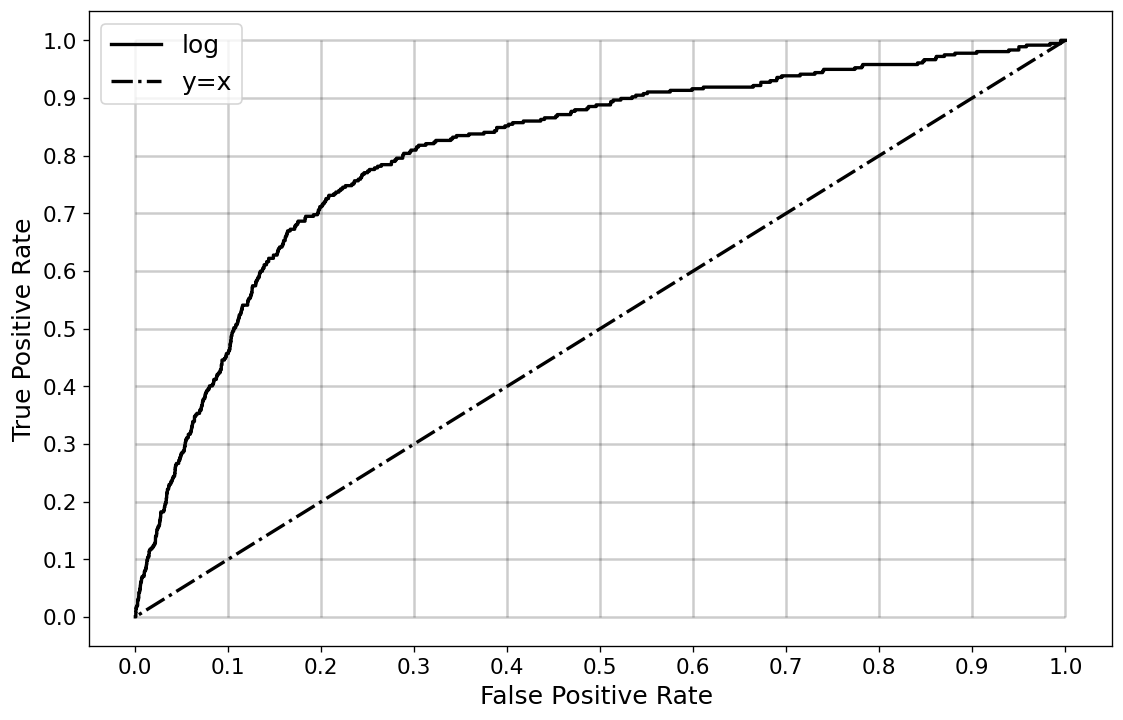
\includegraphics[width=\textwidth]{../img/ROC.png}
    \caption[ROC curve]{The ROC curve for the Logistic Regression Model. This plot is created by choosing every possible binning threshold, evaluating FPR and TPR, then moving on to the next threshold. The plot consists of only the (FPR, TPR) points. FPR (False Positive Rate) is the proportion of false positives to total ground truth negatives. TPR (True Positive Rate) is the proportion of true positives to the total ground truth positives. AUC (Area Under the Curve) is 0.814.}
    \label{fig:ROC}
\end{figure}
\red{REMOVE GRAPHICS BEFORE SUBMISSION}

\begin{table}[htb]
    \centering
    \begin{tabular}{ccccccc}
        \toprule
        Threshold &   TPR &   FPR & PPV & Accuracy &  Balanced Accuracy & F-1 Score \\
        \midrule
        0.500 & 0.000 & 0.000 & 0.000 &     0.996 &     0.500 &   - \\
        0.003 & 0.715 & 0.192 & 0.715 &     0.807 &     0.761 & 0.715 \\
        0.002 & 0.778 & 0.255 & 0.778 &     0.745 &     0.762 & 0.778 \\
        0.002 & 0.901 & 0.532 & 0.901 &     0.470 &     0.684 & 0.901 \\
        0.002 & 0.921 & 0.566 & 0.921 &     0.436 &     0.677 & 0.921 \\
        \bottomrule
    \end{tabular}
    \caption{Selected thresholds and their corresponding performance metrics. These (FPR, TPR) points are shown in the ROC plot shown in Fig \ref{fig:ROC}. TPR (True Positive Rate) is also referred to as Sensitivity, Recall, and Hit Rate. FPR (False Positive Rate) is also referrred to as Fallout Rate. PPV (Positive Predictive Value) is also referred to as Precision.}
    \label{tbl:performance}
\end{table}

In order to make the results of this study comparable to other homelessness prediction studies, the results of our model evaluated at the threshold where the TPR is near the levels listed in the other studies are shown in Table \ref{tbl:performance}. Each row in Table \ref{tbl:performance} represents a single (FPR, TPR) point on the ROC curve in Fig~\ref{fig:ROC}. 

\begin{table}[!h]
    \begin{tabular}{lcccc}
    \toprule
              Feature &  Mean Coeff &  Mean OR &  Mean [0.025 &  Mean 0.975] \\
    \midrule
    PAST\_DUE &       0.309 &    1.362 &        1.351 &        1.373 \\
    TOTAL\_CUR\_BALANCE &       0.000 &    1.000 &        1.000 &        1.000 \\
     NUM\_PREM\_FOR\_PER &      -6.236 &    0.002 &        0.002 &        0.002 \\
    BREAK\_ARRANGEMENT &       0.494 &    1.639 &        1.486 &        1.807 \\
     NUM\_PER\_FOR\_PREM &      -0.145 &    0.865 &        0.819 &        0.913 \\
    \bottomrule
    \end{tabular}
    \caption{Mean logistic model coefficient (Coeff), mean odds ratio (OR), and mean 95\% confidence interval for the odds ratio for each model feature over all folds. Odds ratio describes how much the predicted odds of an event will increase if a single variable is increased by one.}
    \label{tbl:meanParams}
\end{table}

The odds ratio for each feature shown in Table \ref{tbl:meanParams} give some idea of the importance of each feature to the logistic model. 

%------------------- DISCUSSION ---------------------------------
\section*{Discussion}
\subsection*{Performance Comparison}
Comparing binary classification models is difficult because their scores in performance metrics differ based on the chosen binning threshold. For the Logistic Regression model, the default threshold of 0.5 is likely not the most appropriate for the use-case of predicting homelessness since homelessness is a rare event. Notice the poor performance of our model at the threshold of 0.5 in Table \ref{tbl:performance}. 

% Call for standardized reporting
So far the related research has published model performances based on the default prediction binning threshold of 0.5 with a variety of performance metrics reported \red{Add citation}. Because in this use-case it is much worse to incur a Type II Error (false negative) than a Type I Error (false positive), model performance and evaluation should focus on a threshold where the True Positive Rate (TPR) is high, meaning most of the positive cases are correctly predicted. This focus on correctly predicting positive cases has been repeatedly pointed out in the literature \cite{vanberlo2021interpretable} \red{ADD SOURCES HERE}. We propose the reporting standard of choosing the binning threshold that produces a TPR as near to 0.90 (90.0\%) as possible, then report False Positive Rate (FPR) and other metrics at the same threshold. A TPR of 0.90 is appropriately high for this use-case. Reporting the FPR allows homelessness prediction programs to asses the cost and savings of the prediction model based on their service population. Reporting the Area Under the Curve for the Receiver Operator Characteristic is another helpful metric to report that provides a measure of model performance at all thresholds \red{Do we care about performance at other thresholds?}. Displaying the ROC plot is also very helpful for comparing models. 

% Compare to previous research
We compare our model to those developed in previous studies by choosing the binning threshold that produces most closely the same TPR as reported by each of the previous studies, then comparing the FPR and Positive Predictive Value (PPV), when given. For the same TPR a lower FPR and higher PPV are preferred. Shinn's Screening Model achieved a TPR of 0.716 with a FPR of 0.657 and no PPV reported \cite{shinn2013efficient}. At the same TPR our model achieved a FPR of 0.192. Byrne's Logistic Regression Model achieved a TPR of 0.778 with a FPR of 0.049 (calculated from reported True Negative Rate: FPR = 1 - TNR) and PPV of 0.117 \cite{byrne2020classification}. At the same TPR our model achieved a FPR of 0.255 and PPV of 0.778. VanBerlo's HIFIS-RNN-MLP Model achieved a TPR of 0.921 and PPV of 0.651 with no FPR reported \cite{vanberlo2021interpretable}. At the same TPR our model achieved a PPV of 0.921.

When comparing our model with the selected previous studies at the same TPR, our model achieved a lower FPR than Shinn's Screening Model, a lower FPR and higher PPV than Byrne's Logistic Model, and a higher PPV than VanBerlo's HIFIS-RNN-MLP Model. The result that our model achieved a higher PPV but a lower FPR than Byrne's Logistic Model indicates that more of our model's predicted positives are true positives but a larger proportion of negatives were falsely predicted as positives by our model. This seems contradictory, especially considering how much higher our PPV is. Byrne's FPR is suspiciously low. \red{Rephrase previous}

\subsection*{Model Usage}
For model use, a specific binning threshold must be chosen with different thresholds yielding different model performance. For HPPs that plan to target a small segment of the population, a high threshold is appropriate so that only a few predictions are binned as positives. High thresholds correspond to the lower left region of the ROC plot where the TPR and the FPR are both low. For HPPs that plan to target large portions of the population, a low threshold, corresponding to the upper right portion of the ROC plot, is appropriate. 

Since the method of K-Folds was employed, $k=4$ models were actually trained and the overall performance is an average of all the models. If similar performance is to be attained, all models must predict the risk of experiencing homelessness for a new person, then the average prediction will be the prediction of the overall method.

\subsection*{Variability of Evaluation}
As mentioned in the Methods Section, model evaluation was highly sensitive to which people were selected for the training set and the test set. The method of K-Folds was employed to mitigate this issue, but evaluation remained variable from run to run because the selection of which people ended up in which fold was random and differed from run to run. This problem is a result of the data imbalance; because the models have so few positive cases to learn from, the makeup of those positive cases is important. If the random split happens to select positive cases for the training set that are different from the test set, then the model will have more difficulty identifying those positive cases in the test set. 

The choice of $k$ also had an effect on model evaluation. Over several runs it was found that the best model performance was achieved from $k=2$ to $k=5$. For balanced datasets, performance is generally increased with increasing $k$ until about $k=10$ where performance does not increase significantly if $k$ is increased further. Training on large datasets, at least 5000 entities, can achieve good results with $k$ values as low as 5. Typically $k=10$ is used by convention \cite{marcot2020optimal}. With imbalanced data, however, if the value of $k$ is large then there are very few positive cases in the test set, so the models have difficulty distinguishing this small set from all the negative cases. This is likely the reason why lower $k$ values were found to produce better performance for this study.

\subsection*{Outcome Variable Selection}
Though the eventual choice of outcome measure was the binary variable of if a person was ever recorded as experiencing homelessness (CMIS\_MATCH), several others were investigated. One was a numerical variable describing the number of months until an individual experienced an episode of homelessness. This seemed promising, but posed the challenge of assigning some value(s) to negative cases. Two more outcome variables investigated were the binary variables recording if an individual was within six months or one month of experiencing an episode of homelessness, respectively. 

The outcome used for modeling was chosen to be the one that had the highest association with the predictor variables based on appropriate association metrics. CMIS\_MATCH had the largest associations with the predictor variables compared to the other potential outcome measures. An interesting result here is that the variables recording if an individual will experience homelessness within six months and one month are associated less with the explanatory variables than CMIS\_MATCH. This seems to indicate that the data used for this project is better at discerning if an individual will ever experience homelessness than it is at discerning either if the individual will experience homelessness within the month or within six months.

\subsection*{Predictor Variable Selection}
\begin{itemize}
    \item selected those that are likely to be widely available across US
    \item no performance change between grouped, ungrouped billing features (interesting bc landlord likely pays some)
\end{itemize}

\subsection*{Dependence on Time}
It was hypothesized that time is an important factor in predicting homelessness. As people get closer in time to experiencing homelessness they are likely to be more distinguishable from the general population. The history in time of a person's characteristics may be an important factor in predicting homelessness. Two approaches were considered to incorporate individual's previous characteristics in predicting the likelihood of homelessness.

The first approach was to generate naive trajectories for each person over time. This was done by fitting a linear line for each variable in time, then only retaining the slope of the line. This method records the long-term trend of a person in each variable over time. These trends were used as predictors instead of the actual variable values. The performance of the models using these trajectories was lower than the methods discussed so far.

Another method investigated for including a person's previous values as predictors was to take the first difference in each variable of the last two months available for each person. These variable differences capture the local changes in people's characteristics. The differences were used as predictors in the place of the original variable values. Again, model performance was lower here than for the main methods described for this project.

The highest performing method found was to treat each person-place-month combination as a separate entity, make a prediction for each entity, then take the maximum risk prediction for each person over all places and months that person appears in the dataset. This seems to indicate the important aspect of each person is their peak risk. Furthermore, because the outcomes of WITHIN\_6\_MO, and LAST\_MO were less correlated with the predictors than CMIS\_MATCH, an individual's peak risk must not occur immediately before losing their utility account or being evicted. 

\red{add that more appropriate methods could be used to deal with time series - LSTM}

\subsection*{Limitations}
% mislabeling of negative cases
The first limitation is the incompleteness of the data. Before any models are run, of all the people in the data labeled as positive, our confidence that they are actually positive is high - they matched someone who was recorded as experiencing homelessness in the Spokane area. Our confidence in the correct labeling of the negative cases, on the other hand, is lower. Some of the cases labeled as negative in the data may, in reality, be positive cases if they did experience homelessness but this was not recorded in the City of Spokane CMIS database. Because some of the negative cases may be positive cases in reality, the model may have predicted them as positive because they have similar characteristics to other positive cases, but that prediction was labelled as incorrect. This is an unknown factor in this data, but it may cause the model performance to appear worse than it actually is. This problem is likely common to the task of predicting homelessness. \red{add citation}

Another point of interest is that the people predicted as positive by the models may be members of a more general at-risk population. The only outcomes we measured were related to homelessness, but the model predictions and the data investigation reveal that many people labeled as negatives have similar characteristics to the positive cases. These False Positives's may be financially stressed or at-risk in other ways, but we did not have data on other types of outcomes to investigate this. \red{add info about Bryne's study - high prediction associated with drug addiction}

% incompleteness of data
Another limitation of the data was not capturing much of the population. The utility billing data was structured to track accounts and ensure the people responsible for those accounts paid their bills on time. The utility company is a private organization and interested in tracking who is paying for each account so this data structure is appropriate for their uses, but it was not convenient for predicting homelessness.

There were often multiple people associated with a single utility account. These were likely people like spouses, parents, cotenants, or landlords. With these multi-person accounts, it was not recorded who, out of the people associated with the account, paid for each bill. For this project it was assumed that the main account holder always paid since they were ultimately financially responsible for the account, but this is likely not always true. There may be useful information regarding who paid a utility bill for each month; specifically, it may be a risk indicator if someone other than the main account holder paid the bill for a given month.

% matching, don't know who pays bills
Avista and City utility billing information was matched using address, not person, so it is unknown if the same person actually paid both bills. This choice was made because matching on address and month across the billing systems of Avista and the City of Spokane had a much higher match rate than matching on the recorded account holder names. It is likely that many of the City utility bills for apartments were paid by the landlord and so would remain unaltered if the tenant was experiencing financial stress. This aspect is addressed, to some degree, by the selection of explanatory variables. It was found that the aggregated measure TOTAL\_60\_DAYS\_AMT, the combined amount owed to Avista and the City for bills over 60 days old, was most associated with the outcome measure out of all other variables related to amount owed. This indicates that even if many landlords did pay consistently for the City utilities even for people who were at risk of homelessness, there was enough information in the amounts owed in City utilities regarding homelessness that aggregating the Avista and City amounts owed produced a variable more strongly associated with CMIS\_MATCH than the individual variables.

% challenges including location
Location was hypothesized to be an important predictor of homelessness, but there were challenges with including location as a predictor in the models. The variables available that contain geographical location information were POSTAL, the person's postal code, BLOCKGROUP\_GEOID, the U.S. Census blockgroup number, and SPA\_PREM\_ID, the assigned identification number for a specific residence. The unit of blockgroup is smaller than that of postal code, but blockgroup areas often do not fall within a single postal code boundary. All of these variables are categorical with POSTAL having 17 unique levels represented in the data, BLOCKGROUP\_GEOID having 279, and SPA\_PREM\_ID having 60785. Because these categorical variables had so many possible values, they could not be incorporated into the logistic model without causing convergence issues.

%------------------- CONCLUSION ---------------------------------
\section*{Conclusion}

%------------------- SUPPORTING INFORMATION ---------------------------------
\section*{Supporting information}


%------------------- ACKNOWLEDGEMENTS ---------------------------------
\section*{Acknowledgements}

\nolinenumbers

% Either type in your references using
% \begin{thebibliography}{}
% \bibitem{}
% Text
% \end{thebibliography}
%
% or
%
% Compile your BiBTeX database using our plos2015.bst
% style file and paste the contents of your .bbl file
% here. See http://journals.plos.org/plosone/s/latex for 
% step-by-step instructions.
% 

%%   Temporary Bibfile included here


\bibliography{PLOS_ONE_MO_Bibliography.bib}
% \bibliographystyle{plos2015.bst}
\bibliographystyle{plain}





\end{document}
